\chapter{Struktura zásuvného modulu}
\label{struktura_pluginu}

\begin{minipage}{0.9\textwidth}
  \dirtree{%
  .1 /.
  .2 data/.
  .3 bpej/.
  .4 \detokenize{SC_BPEJ.csv}.
  .3 icons/.
  .4 checkanalysis.png.
  .4 edit.png.
  .4 loadvfk.png.
  .3 qml/.
  .4 PAR.qml.
  .4 perimeter.qml.
  .3 sql/.
  .4 \detokenize{add_pu_columns_PAR.sql}.
  .4 \detokenize{check_gc_srs.sql}.
  .4 \detokenize{check_pu_columns_PAR.sql}.
  .4 \detokenize{create_fill_gc_srs.sql}.
  .4 \detokenize{create_sobr_spol.sql}.
  .2 pubin/.
  .2 \detokenize{__init__.py}.
  .2 metadata.txt.
  .2 puplugin.cfg.
  .2 puplugin.png.
  .2 puplugin.py.
  .2 puplugin.svg.
  }
\end{minipage}

\begin{description}
	\item[\texttt{data}:] Složka obsahující všechna data.
	\begin{description}[leftmargin=1cm]
		\item[\texttt{bpej}:] Složka obsahující data
pro~analýzu \textit{oceňování podle BPEJ}.
		\begin{description}[leftmargin=1cm]
			\item[\texttt{\detokenize{SC_BPEJ.csv}}:]
Číselník \zk{BPEJ}.
		\end{description}
		\item[\texttt{icons}:] Složka obsahující ikony
záložek.
		\begin{description}[leftmargin=1cm]
			\item[\texttt{checkanalysis.png}:] Ikona
záložky \textit{Kontroly a analýzy}.
			\item[\texttt{edit.png}:] Ikona záložky
\textit{Editace}.
			\item[\texttt{loadvfk.png}:] Ikona záložky
\textit{Načtení VFK souboru}.
		\end{description}
		\item[\texttt{qml}:] Složka obsahující QML soubory.
		\begin{description}[leftmargin=1cm]
			\item[\texttt{PAR.qml}:] QML soubor pro~vrstvu
\texttt{\zk{PAR}}.
			\item[\texttt{perimeter.qml}:] QML soubor
pro~vrstvu obvodu.
		\end{description}
		\item[\texttt{sql}:] Složka obsahující SQL dávky.
		\begin{description}[leftmargin=1cm]
			\item[\texttt{\detokenize{add_pu_columns_PAR.sql}}:]
SQL dávka pro přidání vlastních sloupců.
			\item[\texttt{\detokenize{check_gc_srs.sql}}:]
SQL dávka pro kontrolu přítomnosti tabulek
\texttt{\detokenize{geo-}}\newline\texttt{\detokenize{metry_columns}}
a~\texttt{\detokenize{spatial_ref_sys}}.
			\item[\texttt{\detokenize{check_pu_columns_PAR.sql}}:]
SQL dávka pro~kontrolu přítomnosti vlastních sloupců.
			\item[\texttt{\detokenize{create_fill_gc_srs.sql}}:]
SQL dávka pro~vytvoření a~naplnění tabulek
\texttt{\detokenize{geometry_columns}}
a~\texttt{\detokenize{spatial_ref_sys}}.
			\item[\texttt{\detokenize{create_sobr_spol.sql}}:]
SQL dávka pro~vytvoření tabulek \zk{SOBR} a~\zk{SPOL}.
		\end{description}
	\end{description}
	\item[\texttt{pubin}:] Složka vytvořeného Python balíčku, více
viz příloha \ref{popis_python_balicku}.
	\item[\texttt{\detokenize{__init__.py}}:] Modul
pro~inicializaci zásuvného modulu.
	\item[\texttt{metadata.txt}:] Soubor obsahující metadata
o~zásuvném modulu.
	\item[\texttt{puplugin.cfg}:] Konfigurační soubor zásuvného
modulu.
	\item[\texttt{puplugin.png}:] Ikona zásuvného modulu
ve~formátu PNG.
	\item[\texttt{puplugin.py}:] Hlavní Python modul zásuvného
modulu.
\end{description}

\chapter{Popis vytvořeného Python balíčku}
\label{popis_python_balicku}

Všechny třídy a~metody balíčku mají svůj vlastní \textit{docstring},
tedy komentář, ve~kterém je stručně napsáno, k~čemu třída či~metoda
slouží, jaké má vstupní hodnoty, jaké vyvolává výjimky a~jaké~hodnoty
vrací. Při~vytváření těchto komentářů bylo vycházeno z~\textit{Google
  Python Style
  Guide}\footnote{\url{https://google.github.io/styleguide/pyguide.html}}.

Plugin se bude dále vyvíjet, proto jsou zde popsány pouze základní
informace, díky kterým je možné se v balíčku a modulech orientovat.

\bigskip

\begin{minipage}{0.9\textwidth}
  \dirtree{%
  .1 pubin/.
  .2 pustack/.
  .3 puca/.
  .4 \detokenize{__init__.py}.
  .4 \detokenize{area_pucawidget.py}.
  .4 \detokenize{bpej_pucawidget.py}.
  .4 \detokenize{distance_pucawidget.py}.
  .4 \detokenize{notinmap_pucawidget.py}.
  .4 \detokenize{notinspi_pucawidget.py}.
  .4 \detokenize{perimeter_pucawidget.py}.
  .4 pucawidget.py.
  .4 \detokenize{unowned_pucawidget.py}.
  .3 \detokenize{__init__.py}.
  .3 \detokenize{checkanalysis_puwidget.py}.
  .3 \detokenize{edit_puwidget.py}.
  .3 \detokenize{execute_thread.py}.
  .3 \detokenize{load_thread.py}.
  .3 \detokenize{loadvfk_puwidget.py}.
  .3 puwidget.py.
  .2 \detokenize{__init__.py}.
  .2 dockwidget.py.	
  .2 stackedwidget.py.
  .2 statusbar.py.
  .2 toolbar.py.
  }
\end{minipage}

\begin{description}
	\item[\texttt{pubin}:] Hlavní Python balíček, který obsahuje
všechny vytvořené moduly.
	\begin{description}[leftmargin=1cm]
		\item[\texttt{pustack}:] Balíček obsahující moduly
všech záložek a~jimi používaných tříd. Třídy záložek dědí z~abstraktní
bázové třídy \texttt{PuWidget} nacházející se v~mo\-dulu
\texttt{puwidget.py}.
		\begin{description}[leftmargin=1cm]
			\item[\texttt{puca}:] Balíček obsahující
moduly záložky \textit{Kontroly a~analýzy}. Písmena \texttt{ca} jsou
zkratkou pro~anglický název záložky~– \texttt{CheckAnalysis}. Všechny
třídy kontrol a~analýz dědí z abstraktní bázové třídy
\texttt{PuCaWidget} nacházející se v~modulu
\texttt{pucawidget.py}. Pro spuštění kontroly nebo~analýzy slouží
metoda \texttt{execute}.
			\begin{description}[leftmargin=1cm]
				\item[\texttt{\detokenize{__init__.py}}:]
Modul pro~inicializaci balíčku.
				\item[\texttt{\detokenize{area_pucawidget.py}}:]
Modul pro~kontrolu \textit{výměra nad~mezní odchylkou}.
				\item[\texttt{\detokenize{bpej_pucawidget.py}}:]
Modul pro~analýzu \textit{oceňování podle BPEJ}.
				\item[\texttt{\detokenize{distance_pucawidget.py}}:]
Modul pro~analýzu \textit{měření vzdálenosti}.
				\item[\texttt{\detokenize{notinmap_pucawidget.py}}:]
Modul pro~kontrolu \textit{není v~mapě}.
				\item[\texttt{\detokenize{notinspi_pucawidget.py}}:]
Modul pro~kontrolu \textit{není v~SPI}.
				\item[\texttt{\detokenize{perimeter_pucawidget.py}}:]
Modul pro~kontrolu \textit{obvodem}.
				\item[\texttt{pucawidget.py}:]
Abstraktní bázová třída, ze~které dědí všechny třídy kontrol a~analýz.
				\item[\texttt{\detokenize{unowned_pucawidget.py}}:]
Modul pro~kontrolu \textit{bez~vlastníka}.
			\end{description}
			\item[\texttt{\detokenize{__init__.py}}:]
Modul pro~inicializaci balíčku.
			\item[\texttt{\detokenize{checkanalysis_puwidget.py}}:]
Modul pro~záložku \textit{Kontroly a~analýzy}.
			\item[\texttt{\detokenize{edit_puwidget.py}}:]
Modul pro~záložku \textit{Editace}.
			\item[\texttt{\detokenize{execute_thread.py}}:]
Modul pro~spouštění procesů editace, kontrol a~ana\-lýz v~samostatném
vlákně.
			\item[\texttt{\detokenize{load_thread.py}}:]
Modul pro~spouštění procesu načítání \zk{VFK} souboru v~samostatném
vlákně.
			\item[\texttt{\detokenize{loadvfk_puwidget.py}}:]
Modul pro~záložku \textit{Načtení VFK souboru}.
			\item[\texttt{puwidget.py}:] Abstraktní bázová
třída, ze~které dědí všechny třídy zálo\-žek.
		\end{description}
		\item[\texttt{\detokenize{__init__.py}}:] Modul
pro~inicializaci balíčku.
		\item[\texttt{dockwidget.py}:] Modul pro~hlavní
grafickou komponentu pluginu.
		\item[\texttt{stackedwidget.py}:] Modul pro~grafickou
komponentu, která obsahuje všechny záložky.
		\item[\texttt{statusbar.py}:] Modul pro~stavový řádek.
		\item[\texttt{toolbar.py}:] Modul pro~ikony
na~přepínání mezi záložkami a~sadu standardních nástrojů programu
QGIS.
	\end{description}
\end{description}

\chapter{Uživatelský manuál}
\label{uzivatelsky_manual}

\section{Instalace}
\label{manual_instalace}

Zásuvný modul není součástí oficiálního repositáře QGIS, přesto ho lze
nainstalovat stejným způsobem jako~jiné pluginy. Stačí do~programu
QGIS přidat repositář laboratoře CTU GeoForAll
Lab\footnote{\url{http://geomatics.fsv.cvut.cz/research/geoforall/}}.

Nejprve tedy otevřete okno \textit{Zásuvné moduly $\rightarrow$
Spravovat a~instalovat zásuvné moduly}.

	\begin{figure}[H] \centering
		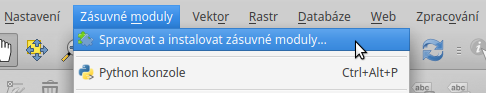
\includegraphics[width=.6\textwidth]{./pictures/instalace-otevreni_okna_zasuvne_moduly.png}
		\caption[Otevření okna \textit{Zásuvné
moduly}]{Otevření okna \textit{Zásuvné moduly} (zdroj: autor)}
		\label{fig:manual_otevreni_okna_zasuvne_moduly}
 	\end{figure}

V~záložce \textit{Nastavení} aktivujte volbu \textit{Zobrazit také
experimentální zásuvné mo\-duly}.

Pomocí tlačítka \textit{Přidat...} doplňte repositář laboratoře
CTU GeoForAll Lab:

\begin{lstlisting}[basicstyle=\footnotesize\ttfamily, backgroundcolor
= \color{light-gray}, numbers=left, columns=fullflexible,
keepspaces=true]
Název:  CVUT GeoForAll Lab
URL:    http://geo.fsv.cvut.cz/geoforall/qgis-plugins.xml
\end{lstlisting}

	\begin{figure}[H] \centering
		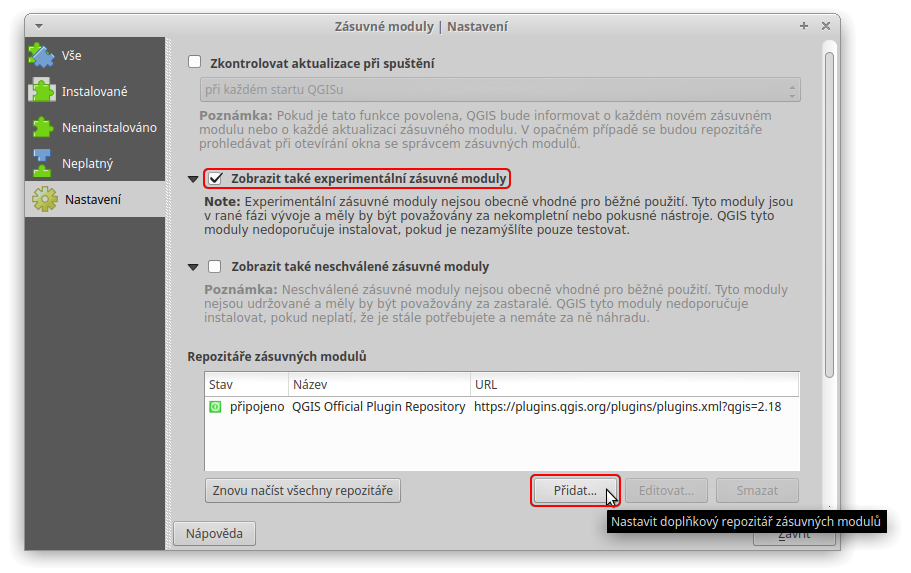
\includegraphics[width=.85\textwidth]{./pictures/instalace-pridani_repositare.png}
		\caption[Přidání repositáře]{Přidání repositáře
(zdroj: autor)}
		\label{fig:manual_pridani_repozitare}
 	\end{figure}
 	
	\begin{figure}[H] \centering
		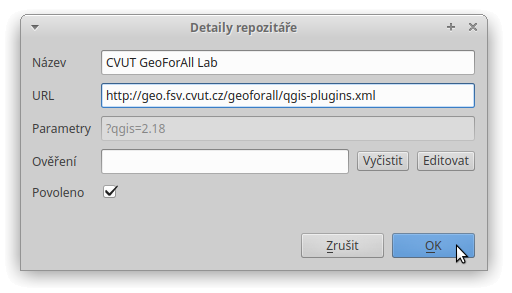
\includegraphics[width=.6\textwidth]{./pictures/instalace-pridani_repositare_geoforall.png}
		\caption[Přidání repositáře GeoForAll Lab]{Přidání
repositáře GeoForAll Lab (zdroj: autor)}
		\label{fig:manual_pridani_repozitare_geoforall_lab}
 	\end{figure}

V záložce \textit{Vše} nebo \textit{Nenainstalované} vyhledejte
\textit{PU Plugin}. Vyberte zásuvný modul a klikněte na
\textit{Instalovat zásuvný modul}.

	\begin{figure}[H] \centering
		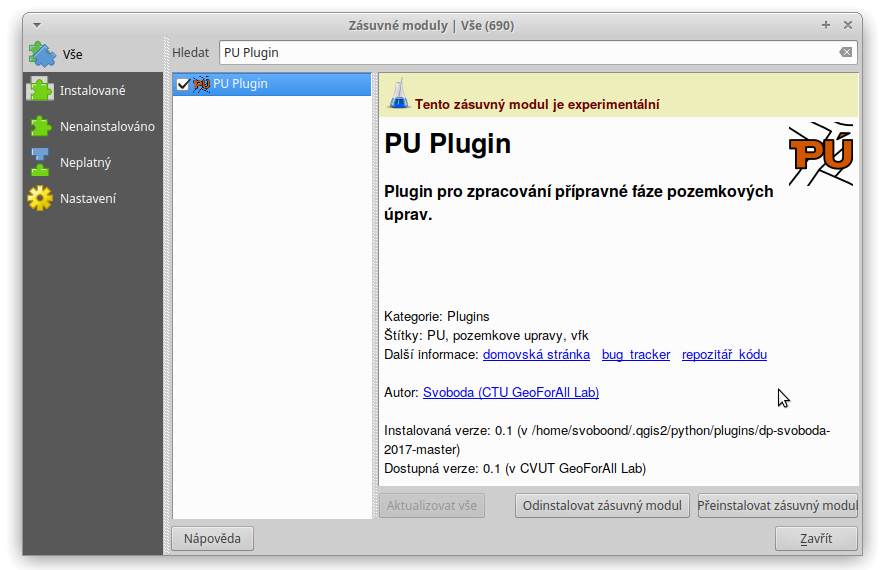
\includegraphics[width=.8\textwidth]{./pictures/instalace-instalace_zasuvneho_modulu.png}
		\caption[Zásuvný modul~– instalace]{Zásuvný modul~–
instalace (zdroj: autor)}
		\label{fig:manual_instalace_puplugin}
 	\end{figure}

Po úspěšném nainstalování se v~\textit{Panelu nástrojů zásuvného
modulu} objeví jeho ikona. Okno zásuvného modulu je možné vyvolat
poklepáním na~jeho ikonu nebo volbou \textit{Zásuvné moduly
$\rightarrow$ PU Plugin $\rightarrow$ PU Plugin}.

	\begin{figure}[H] \centering
		
\includegraphics[width=.4\textwidth]{./pictures/instalace-toolbar.png}
		\caption[Ikona zásuvného modulu v panelu
nástrojů]{Ikona zásuvného modulu v panelu nástrojů (zdroj: autor)}
		\label{fig:manual_ikona_v_panelu_nastroju}
 	\end{figure}

\section{Grafické uživatelské rozhraní}
\label{manual_gui}

	\begin{figure}[H] \centering
		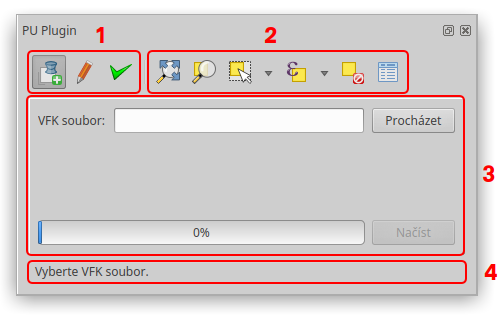
\includegraphics[width=.55\textwidth]{./pictures/main_gui.png}
		\caption[Zásuvný modul~– grafické uživatelské
rozhraní]{Zásuvný modul~– grafické uživatelské rozhraní (zdroj:
autor)}
		\label{fig:manual_main_gui}
 	\end{figure}

\begin{description}
	\item[Prvek 1:] Skupina tří ikon pro~přepínání mezi záložkami:
	\begin{itemize}[leftmargin=1.5cm, noitemsep]
		\item \img{./pictures/loadvfk.png} \textit{Načtení VFK
souboru}
		\item \img{./pictures/edit.png} \textit{Editace}
		\item \img{./pictures/checkanalysis.png}
\textit{Kontroly a analýzy}
 	\end{itemize}
	\item[Prvek 2:] Skupina nástrojů, které jsou propojené
se~standardními nástroji programu QGIS.
	\item[Prvek 3:] Okna záložek zobrazující se v~závislosti
na~tom, která ze~tří ikon záložek (prvek~1) je aktivní.
	\item[Prvek 4:] Stavový řádek, ve~kterém se ukazují zprávy.
\end{description}

\newpage

\section{Komunikace s uživatelem}
\label{manual_komunikace}

Zásuvný modul komunikuje s~uživatelem třemi způsoby:

\begin{enumerate}[leftmargin=1.5cm, noitemsep]
	\item \underline{Stavový řádek} (viz prvek~4
obr.~\ref{fig:manual_main_gui}) představuje nejčastější způsob
zobrazování zpráv zásuvného modulu. Když nevíte jak postupovat, zde
s~největší pravděpodobností najdete potřebné informace. Běžné zprávy
mají černou barvu písma, důležité zprávy se~zobrazují červeně (viz
obr.~\ref{fig:manual_dulezita_zprava}).
	
	\begin{figure}[H] \centering
		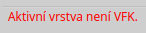
\includegraphics[width=.23\textwidth]{./pictures/statusbar-red_message.png}
		\caption[Stavový řádek~– důležitá zpráva]{Stavový
řádek~– důležitá zpráva (zdroj: autor)}
		\label{fig:manual_dulezita_zprava}
 	\end{figure}

	\item \underline{Pole zpráv} je standardní způsob komunikace
programu QGIS s~uživatelem. Zobrazuje pole v~horní části
mapového okna, které může být nastaveno tak, že po~určité době samo
zmizí, nebo vyžaduje manuální zavření. Zásuvný modul využívá této
komunikace pouze pro~zobrazení významných zpráv, které by neměly být
uživatelem opomenuty (viz obr. \ref{fig:manual_zprava_pole_zprav}).

	\begin{figure}[H] \centering
		
\includegraphics[width=.7\textwidth]{./pictures/message_bar-message.png}
		\caption[Pole zpráv~– zpráva upozornění]{Pole zpráv~–
zpráva upozornění (zdroj: autor)}
		\label{fig:manual_zprava_pole_zprav}
 	\end{figure}

	\item \underline{Logování} je posledním prostředkem
pro~předávání informací, který zásuvný modul používá. Informace
v~anglickém jazyce, zejména chybové hlášky, zapisuje do~vlastní
záložky s~názvem \textit{PU Plugin} (viz
obr.~\ref{fig:manual_logovaci_panel}). Panel logovacích zpráv lze
zobrazit kliknutím na~ikonu \img{./pictures/log.png} v~pravém dolním
rohu QGISu.

	\begin{figure}[H] \centering
		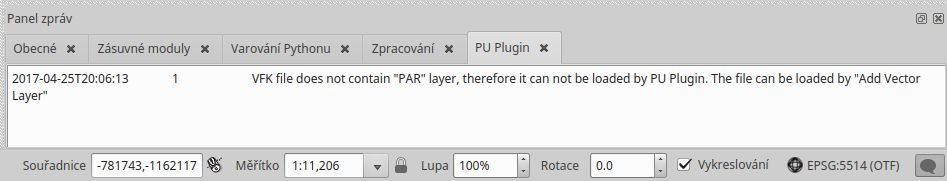
\includegraphics[width=1.0\textwidth]{./pictures/log_panel.png}
		\caption[Panel logovacích zpráv]{Panel logovacích
zpráv (zdroj: autor)}
		\label{fig:manual_logovaci_panel}
 	\end{figure}

\end{enumerate}

\newpage

\section{Načtení VFK souboru}
\label{manual_nacteni_vfk}

Záložka \textit{Načtení VFK souboru} slouží k~načtení vrstvy parcel
ze~souboru~\zk{VFK}.

	\begin{figure}[H] \centering
		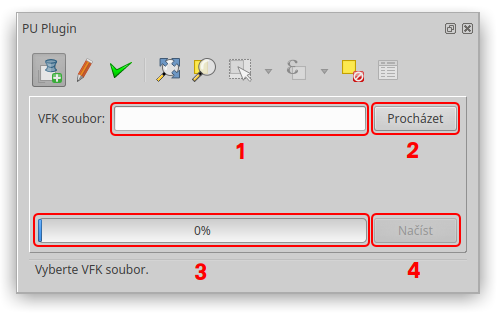
\includegraphics[width=.55\textwidth]{./pictures/nacteni_vfk_gui.png}
		\caption[Záložka \textit{Načtení VFK souboru}~–
grafické uživatelské rozhraní]{Záložka \textit{Načtení VFK souboru}~–
grafické uživatelské rozhraní (zdroj: autor)}
		\label{fig:manual_nacteni_vfk_gui}
 	\end{figure}

\begin{description}
	\item[Prvek 1:] Textové pole pro~cestu k~\zk{VFK} souboru.
	\item[Prvek 2:] Tlačítko pro~zobrazení dialogového okna
pro~procházení adresářů. Filtruje soubory s~příponou \textit{*.vfk},
pamatuje si poslední použitou cestu.
	\item[Prvek 3:] Indikátor průběhu načítání \zk{VFK} souboru.
	\item[Prvek 4:] Tlačítko pro~načítání \zk{VFK}
souboru. Aktivuje se pouze v~případě, že textové pole (prvek~1)
obsahuje cestu k~existujícímu \zk{VFK} souboru.
\end{description}

\subsection{Postup}
\label{manual_nacteni_postup}

Nejprve je zapotřebí zvolit \zk{VFK} soubor, který chcete načíst. To
lze udělat dvěma způsoby. Buď kliknete na~tlačítko \textit{Procházet}
(prvek~2), vyberete požadovaný soubor a~cesta k~souboru se automaticky
zapíše do~textového pole (prvek~1), nebo zkopírujete cestu k~\zk{VFK}
souboru přímo do~zmíněného textové pole.

Když se v~textovém poli nachází cesta k~validnímu \zk{VFK} souboru,
aktivuje se tlačítko \textit{Načíst} (prvek~4) a~můžete zahájit
import.

O~průběhu načítání vás informuje indikátor průběhu (prvek~3) a~zprávy
ve~stavovém řádku.

\subsection{Symbologie vrstvy parcel}
\label{manual_nacteni_symbologie}

Symbologie načtené vrstvy parcel se řídí podle druhu pozemku. Při
měřítku 1:4000 a~větším přiblížení se zobrazí parcelní čísla.

	\begin{figure}[H] \centering
		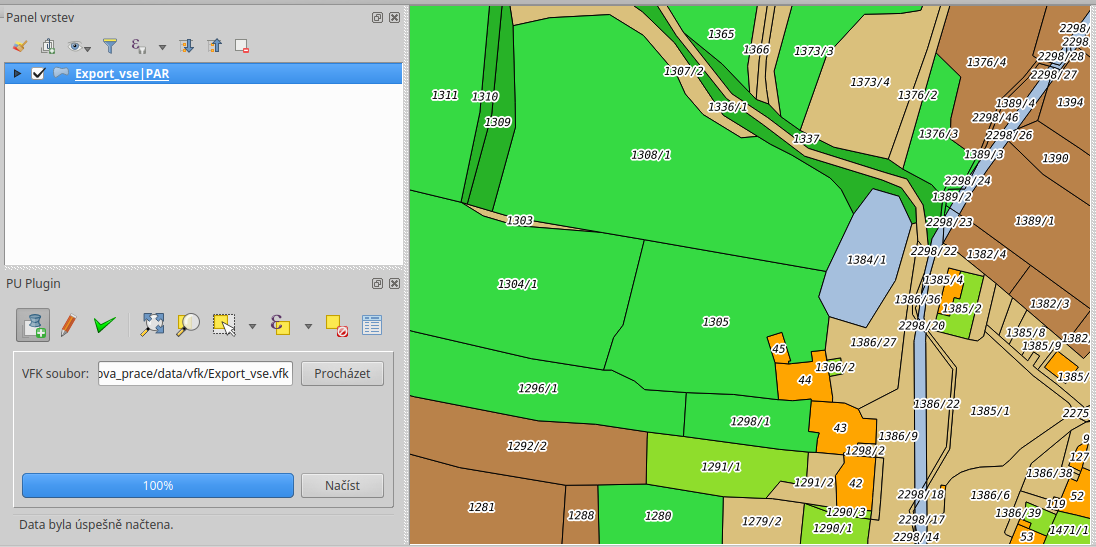
\includegraphics[width=.9\textwidth]{./pictures/symbologie_par.png}
		\caption[Vrstva parcel~– symbologie]{Vrstva parcel~–
symbologie (zdroj: autor)}
		\label{fig:manual_symbologie_par}
 	\end{figure}

\subsection{Atributová tabulka vrstvy parcel}
\label{manual_nacteni_tabulka}

Zásuvný modul v~atributové tabulce kvůli přehlednosti skrývá všechny
nepotřebné sloupce. Pro~větší srozumitelnost mají viditelné sloupce
aliasy.

	\begin{figure}[H] \centering
		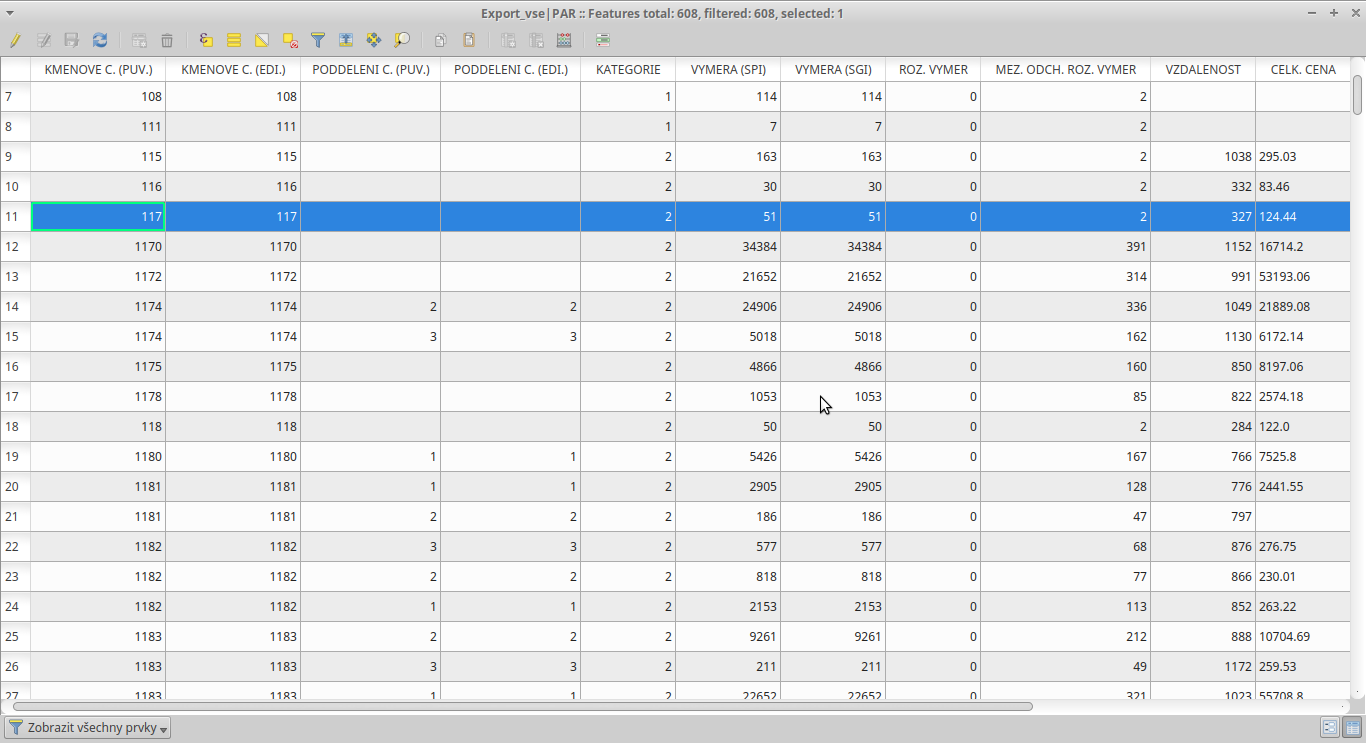
\includegraphics[width=.95\textwidth]{./pictures/nacteni-tabulka.png}
		\caption[Vrstva parcel~– atributová tabulka]{Vrstva
parcel~– atributová tabulka (zdroj: autor)}
		\label{fig:manual_tabulka_par}
 	\end{figure}

\newpage

\section{Editace}
\label{manual_editace}

Po úspěšném nahrání vrstvy parcel lze začít s~editací. Záložka
\textit{Editace} poskytuje nástroje k~úpravě geometrie a~zařazení
parcel do~kategorií.

	\begin{figure}[H] \centering
		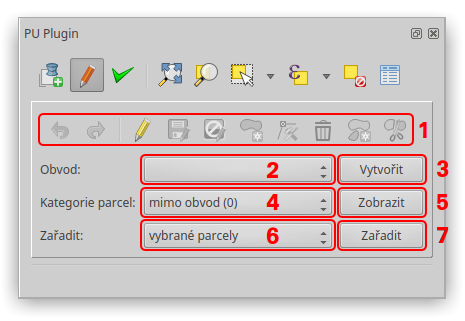
\includegraphics[width=.55\textwidth]{./pictures/editace_gui.png}
		\caption[Záložka \textit{Editace}~– grafické
uživatelské rozhraní]{Záložka \textit{Editace}~– grafické uživatelské
rozhraní (zdroj: autor)}
		\label{fig:manual_editace_gui}
 	\end{figure}

\begin{description}
	\item[Prvek 1:] Skupina nástrojů pro~editaci, které jsou
propojené se~standardními nástro\-ji programu QGIS.
	\item[Prvek 2:] Rozbalovací menu s~aktuálně načtenými
polygonovými vrstvami.
	\item[Prvek 3:] Tlačítko pro~zobrazení dialogového, ve~kterém
lze zvolit adresář a~název vrstvy obvodu. Filtruje soubory s~příponou
\textit{*.shp}, pamatuje si poslední použitou cestu.
	\item[Prvek 4:] Rozbalovací menu s~kategoriemi
parcel. Na~výběr jsou tyto kategorie, číslo v~závorce udává hodnotu,
kterou zásuvný modul pro~kategorii používá:
	\begin{itemize}[leftmargin=1.5cm, noitemsep]
		\item \textit{mimo obvod (0)}
		\item \textit{v~obvodu~– neřešené (1)}
		\item \textit{v~obvodu~– řešené (2)}
		\item \textit{bez kategorie}
	\end{itemize}
	\item[Prvek 5:] Tlačítko pro~zobrazení (výběr) parcel
v~aktuálně zvolené kategorii.
	\item[Prvek 6:] Rozbalovací menu s~variantami zařazení
parcel. K~dispozici jsou dvě možnosti:
	\begin{itemize}[leftmargin=1.5cm, noitemsep]
		\item \textit{vybrané parcely}~– zařadí vybrané
parcely do~aktuálně zvolené kategorie.
		\item \textit{obvodem}~– zařadí všechny parcely
do~kategorií na~základě obvodu.
	\end{itemize}
	\item[Prvek 7:] Tlačítko pro~provedení zařazení.
\end{description}

\subsection{Postup}
\label{manual_editace_postup}

Zásuvný modul pracuje s~aktivní vrstvou, tj. vrstva vybraná v~panelu
vrstev, který se ve~výchozím nastavení nachází na~levé straně okna.

Vrstvu parcel můžete editovat pomocí sady standardních nástrojů
v~horní části pluginu (prvek~1).

Nejdůležitější funkcionalitou této záložky je ovšem zařazení parcel
do~kategorií. Aby bylo na~první pohled zřejmé, ve~které kategorii jsou
jednotlivé parcely zařazeny, používá zásuvný modul tzv.~vrstvu
obvodu. Jedná se o~samostatnou vrstvu ve~formátu
\textit{Esri Shapefile}. Adresář a~název této vrstvy můžete specifikovat
pomocí tlačítka \textit{Vytvořit} (prvek~3). Po~poklepání na~zmíněné
tlačítko se otevře dialogové okno, kde lze zvolit umístění vrstvy
obvodu. Z~aktivní vrstvy, která musí být \zk{VFK}, se vytvoří vrstva
obvodu, zásuvný modul ji načte a~vybere v~rozbalovacím menu (prvek~2).

Pokud cesta k~vrstvě obvodu není definována (rozbalovací menu je
prázdné), nebo je v~rozbalovací menu vybrána vrstva, která nebyla
vytvořena zásuvným modulem a~tudíž neobsahuje potřebné sloupce, plugin
automaticky vytvoří vrstvu obvodu ve~stejném adresáři, ve~kterém se
nachází aktivní vrstva parcel.

Funkce pro~vytvoření obvodu je volána v~momentě, kdy je pro~vrstvu
%%% ML: ulozena zmena je dvakrat ve stejne vete, preformulovat
% OS: Zmeneno.
parcel uložena změna geometrie, potvrzena editace, při~které došlo
k~vymazání prvku, nebo je pomocí tlačítka \textit{Zařadit} (prvek~7)
provedeno zařazení parcel.

Zásuvný modul nabízí dvě varianty zařazení parcel (prvek~6). První
možností je volba \textit{vybrané parcely}, která provede zařazení
vybraných parcel do~zvolené kategorie (prvek~4).

Druhý způsob nazvaný \textit{obvodem} rozřadí všechny parcely
ve~\zk{VFK} vrstvě do~ka\-tegorií. Jako podklad použije aktuálně
vybranou vrstvu obvodu (viz prvek~2). Tato varianta pracuje pouze
s~obvody, které vytvořil zásuvný modul pro~pozemkové
úpravy. Pro~zařazení do~kategorie musí být parcela kompletně uvnitř
geometrie příslušného prvku obvodu.

Pro kontrolu nabízí zásuvný modul tlačítko \textit{Zobrazit}
(prvek~5), které vybere, a~tím pádem zvýrazní, prvky v~kategorii.

Pokud vytvoříte novou parcelu, nebo~pomocí nástroje \textit{Přidat
  část} doplníte popis\-né údaje o~geometrii, vyplňte měřítko podkladů
%%% ML: ta tecka je soucasti nazvu sloupce, to je divne?
% OS: Je to soucasti aliasu sloupce.
do~sloupce \textit{MERITKO PODKL.}. Tento údaj používá kontrola
\textit{výměra nad mezní odchylkou}.

\subsection{Symbologie vrstvy obvodu}
\label{manual_editace_symbologie}

Pro symbologii vrstvy obvodu byla zvolena červená barva, popisky
obsahují pouze číslo kategorie.

	\begin{figure}[H] \centering
		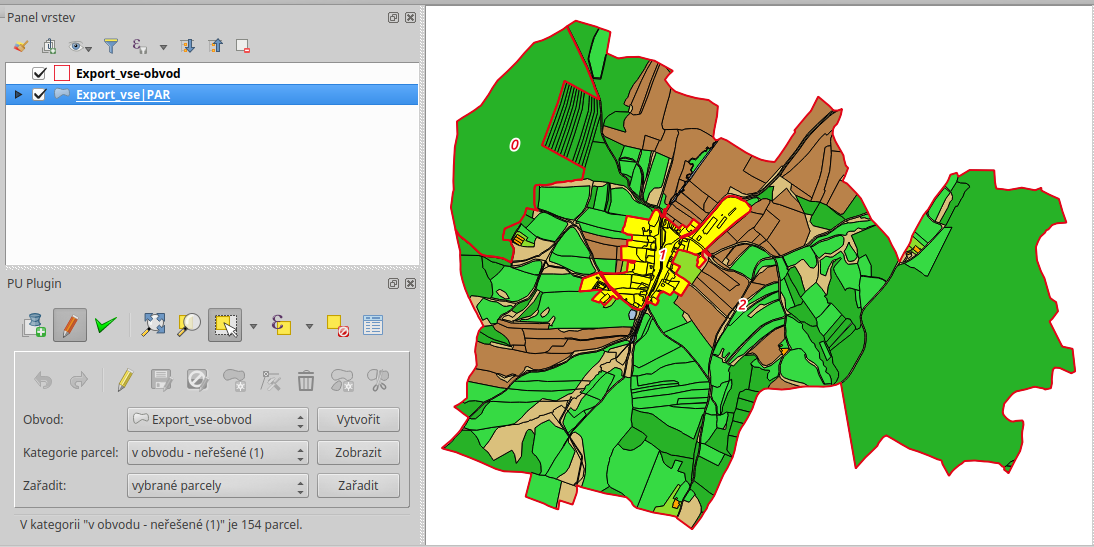
\includegraphics[width=1.0\textwidth]{./pictures/symbologie_obvod.png}
		\caption[Vrstva obvodu~– symbologie]{Vrstva obvodu~–
symbologie (zdroj: autor)}
		\label{fig:manual_symbologie_obvod}
 	\end{figure}

\subsection{Atributová tabulka vrstvy obvodu}
\label{manual_editace_tabulka}

Vrstva obvodu se vytváří z~vrstvy parcel, ovšem pouze informace o
kategorii je pro obvod relevantní. Z~toho důvodu je viditelný pouze
sloupec \texttt{KATEGORIE}.

	\begin{figure}[H] \centering
		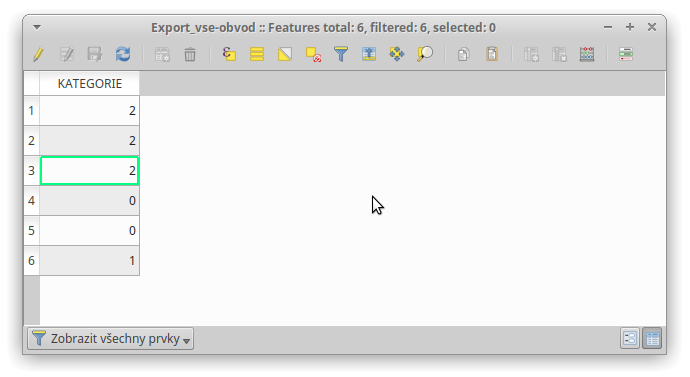
\includegraphics[width=.7\textwidth]{./pictures/editace-tabulka.png}
		\caption[Vrstva obvodu~– atributová tabulka]{Vrstva
obvodu~– atributová tabulka (zdroj: autor)}
		\label{fig:manual_tabulka_obvod}
 	\end{figure}

\newpage

\section{Kontroly a analýzy}
\label{manual_kontroly_analyzy}

Poslední záložka zásuvného modulu nabízí možnost zkontrolovat data,
zejména soulad mezi~\zk{SPI} a~\zk{SGI}, a~provést analýzy nezbytné
pro~sestavení nárokových listů.

	\begin{figure}[H] \centering
		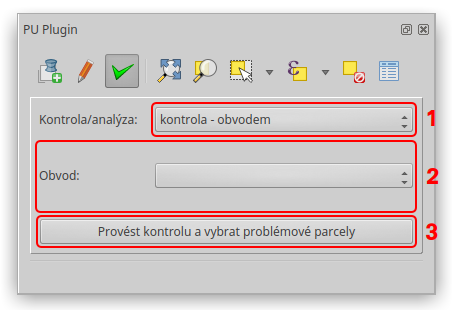
\includegraphics[width=.55\textwidth]{./pictures/ca_gui.png}
		\caption[Záložka \textit{Kontroly a analýzy}~–
grafické uživatelské rozhraní]{Záložka \textit{Kontroly a analýzy}~–
grafické uživatelské rozhraní (zdroj: autor)}
		\label{fig:manual_ca_gui}
 	\end{figure}

\begin{description}
	\item[Prvek 1:] Rozbalovací menu pro~přepínání mezi kontrolami
a~analýzami.
	\item[Prvek 2:] Okna kontrol a~analýz zobrazující se
v~závislosti na~tom, která položka rozbalovacího menu (prvek~1) je
vybrána.
	\item[Prvek 3:] Tlačítko pro~provedení kontroly či~analýzy.
\end{description}

V~rozbalovacím menu (prvek~1) zvolte kontrolu či~analýzu, důsledkem
čehož se změní dolní okno (prvek~2). Když je vše potřebné zadané, lze
kontrolu či~analýzu spustit. Zprávy ve~stavovém řádku poskytují
informace o~výsledku.

\subsubsection{Kontrola~– obvodem}
\label{manual_kontrola_obvodem}

Kontrola obvodem provádí výběr parcel, které nejsou kompletně uvnitř
vrstvy obvodu.

Jestliže od~začátku pracujete pouze s~jednou vrstvou obvodu, měl by
být výsledek této kontroly stejný jako při~zvolení kategorie
\textit{bez kategorie} (prvek~4 na~obr.~\ref{fig:manual_editace_gui})
a~provedení výběru prvků v~kategorii pomocí tlačítka \textit{Zobrazit}
(prvek~5 na~obr.~\ref{fig:manual_editace_gui}). Lišit se tyto dvě
metody budou v~momentě, kdy si do~QGISu nahrajete vrstvu obvodu,
kterou jste vytvořili s~jinou vrstvou parcel. Jinými slovy tato
kontrola používá geometrii vrstvy obvodu a~tlačítko \textit{Zobrazit}
v~záložce \textit{Editace} vybírá parcely na~základě údajů uložených
v~atributové tabulce.

Jediným potřebným vstupem je zmiňovaná vrstva obvodu v~rozbalovacím
menu (viz obr.~\ref{fig:manual_kontrola_obvodem_gui}), které je
propojené s~menu vrstvy obvodu v~záložce \textit{Editace}.

	\begin{figure}[H] \centering
		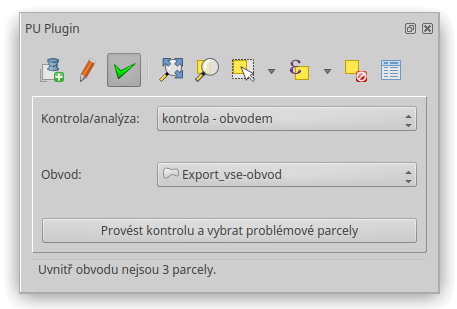
\includegraphics[width=.55\textwidth]{./pictures/kontrola-obvodem.png}
		\caption[Kontrola \textit{obvodem}~– grafické
uživatelské rozhraní]{Kontrola \textit{obvodem}~– grafické uživatelské
rozhraní (zdroj: autor)}
		\label{fig:manual_kontrola_obvodem_gui}
 	\end{figure}

\subsubsection{Kontrola~– není v SPI}
\label{manual_kontrola_neni_v_spi}

Kontrola \textit{není v SPI} slouží k~zobrazení parcel, které nejsou
v~souboru popisných informací.

\subsubsection{Kontrola~– není v mapě}
\label{manual_kontrola_neni_v_mape}

Kontrola \textit{není v~mapě} vybírá parcely, které mají nulovou
geometrii a~tudíž se nezobrazují v~mapovém okně.

\subsubsection{Kontrola~– výměra nad mezní odchylkou}
\label{manual_kontrola_vymera}

Kontrola \textit{výměra nad~mezní odchylkou} ověřuje, zda~rozdíl mezi
výměrou dle~\zk{SPI} a~výměrou vypočtenou z~\zk{SGI} nepřekračuje
mezní odchylku. Ta je stanovena kata\-strální vyhláškou a~závisí na~kódu
kvality nejméně přesně určeného lomového bodu na~hranici
parcely. Jestliže je parcela digitalizovaná, kód kvality podrobných
bodů se určí podle~měřítka podkladové mapy (viz sloupec
\texttt{MERITKO PODKL.}).

\subsubsection{Kontrola~– bez vlastníka}
\label{manual_kontrola_bez_vlastnika}

Kontrola \textit{bez~vlastníka} vybírá parcely, které jsou
bez~vlastníka, tzn. že~nemají přiřazený list vlastnictví.

\subsubsection{Analýza~– měření vzdálenosti}
\label{manual_analyza_vzdalenosti}

Analýza \textit{měření vzdálenosti} počítá pro~všechny řešené parcely
vzdálenost jejich těžiště od~referenčního bodu. Výsledné zaokrouhlené
hodnoty v~metrech ukládá do sloupce \texttt{VZDALENOST}.

Pro~spuštění této kontroly je zapotřebí v~rozbalovacím menu, které
filtruje bodové vrstvy, zvolit vrstvu referenčního bodu, viz
obr.~\ref{fig:manual_analyza_vzdalenosti_gui}. Vybraná vrstva
referenčního bodu musí obsahovat právě jeden prvek a~musí mít stejný
souřadnicový systém jako vrstva parcel.

	\begin{figure}[H] \centering
		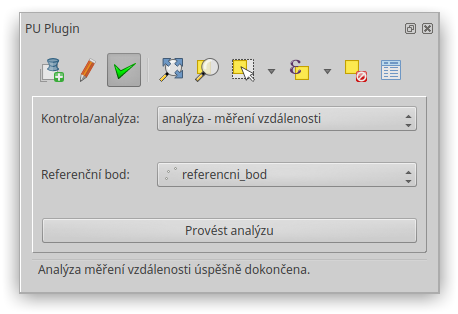
\includegraphics[width=0.55\textwidth]{./pictures/analyza_vzdalenost.png}
		\caption[Analýza \textit{měření vzdálenosti}~–
grafické uživatelské rozhraní]{Analýza \textit{měření vzdálenosti}~–
grafické uživatelské rozhraní (zdroj: autor)}
		\label{fig:manual_analyza_vzdalenosti_gui}
 	\end{figure}

\subsubsection{Analýza~– oceňování podle BPEJ}
\label{manual_analyza_bpej}

Analýza \textit{oceňování podle BPEJ} počítá cenu pozemku na~základě
vrstvy hranic \zk{BPEJ}.

	\begin{figure}[H] \centering
		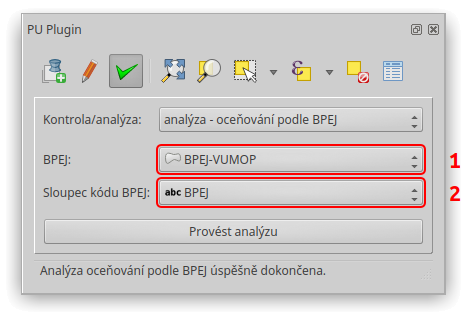
\includegraphics[width=0.55\textwidth]{./pictures/analyza_bpej.png}
		\caption[Analýza \textit{oceňování podle BPEJ}~–
grafické uživatelské rozhraní]{Analýza \textit{oceňování podle BPEJ}~–
grafické uživatelské rozhraní\newline (zdroj: autor)}
		\label{fig:manual_analyza_bpej_gui}
 	\end{figure}

\begin{description}
	\item[Prvek 1:] Rozbalovací menu s~aktuálně načtenými
polygonovými vrstvami.
	\item[Prvek 2:] Rozbalovací menu se~sloupci vybrané vrstvy
\zk{BPEJ}.
\end{description}

Vyberte vrstvu hranic \zk{BPEJ} (prvek~1) a~poté zvolte sloupec,
ve~kterém jsou uloženy kódy \zk{BPEJ}. Vrstva hranic \zk{BPEJ} musí
mít stejný souřadnicový systém jako vrstva parcel.

Pro určení ceny za~metr čtvereční jednotlivých kódů \zk{BPEJ} analýza
používá číselník \zk{BPEJ} z~Českého úřadu zeměměřičského
a~katastrálního.

Do~atributové tabulky se zapíše nejen cena celková (sloupec
%%% ML: opet tecka v nazvu sloupce (aaa, uz to mam, to je alias :-)...
\texttt{CELK. CENA}), ale~také cena za~metr čtvereční, výměra a~cena
dle jednotlivých bonit v~příslušné parcele (sloupec \texttt{BPEJ
KOD-CENA ZA M2-VYMERA-CENA}).

Pokud omylem zvolíte špatný slou\-pec, nebo když kód \zk{BPEJ} není
nalezen v~číselníku, zásuvný modul vybere ve~vrstvě obvodu prvky,
pro~které nenalezl ceny, a~informuje vás o~problému.
